\section{Methods}\label{sec:methods}

\subsection{Study design}\label{subsec:design}

The protocol implements an observational, prospective, longitudinal study with repeated measures, conducted over four consecutive months in one secondary school. No educational intervention is delivered; ordinary teaching is preserved at all times. Recordings take place in a single instrumented reference classroom during the four weekly Mathematics sessions of one 3rd-of-ESO group (group A) and during the weekly Mathematics sessions of a second 3rd–4th-of-ESO group used as the comparison condition. \textcolor{blue}{The comparison group receives the same teacher annotation, end-of-session rating, monthly PVT, and session-level covariates as the instrumented group, but is not equipped with wearable or EEG sensors, is not recorded on video, and does not host the environmental sensing platform. This design provides a within-school reference for the label and PVT distributions under ordinary teaching conditions, against which the instrumented group's multimodal data can be descriptively compared.} The four-month duration provides sufficient longitudinal coverage to characterise within-subject signal stability across a full school trimester and satisfies the minimum exposure required to attenuate Psychomotor Vigilance Task practice effects at the monthly cadence \parencite{Basner2018_pvt_practice}. The unit of analysis is the 5-minute time window. The total sample size is determined by class-complete enrolment in the instrumented group plus consent uptake in the comparison group; the exact $n$ is fixed at the start of the consent campaign and reported alongside the data-release manifest.

\subsection{Setting and population}\label{subsec:population}

The study is conducted in a single secondary school in Albacete (Castilla-La Mancha, Spain). Eligible participants are students enrolled in the 3rd and 4th years of compulsory secondary education (ESO), aged 14--16. The instrumented group is one 3rd-of-ESO class (group A) recorded during its four weekly Mathematics sessions. The comparison group is a second class of the same school year recorded during its weekly Mathematics sessions. Recruitment is class-complete: every student in either group is eligible to participate; non-participants attend the lesson normally and their data are never recorded, processed or stored. The participating school is selected for its willingness to host a four-month multimodal-monitoring deployment of minors and for the logistical fit of the instrumented reference classroom with the platform's spatial requirements; the team acknowledges and discusses the resulting host-school selection effect in \Cref{subsec:limitations} of the Discussion.

\subsection{Recruitment, consent and assent}\label{subsec:recruitment}

Participation requires \emph{both} (a) written informed consent from each participant's parent or legal guardian and (b) written assent from the minor. The minor's refusal overrides any parental authorisation; the parent's refusal overrides participation regardless of the minor's preference. Consent and assent are obtained on paper, archived under restricted access by the principal investigator, and may be withdrawn at any time without justification. Withdrawal triggers the immediate cessation of data collection for that participant and the full deletion of their previously collected data; the deletion event is recorded in the data-governance log (\Cref{sec:appendix-privacy}). Neither participation nor non-participation has any consequence whatsoever for academic evaluation, school progression, or teacher--student relationships. No individual feedback from the study is shared with the school, the families, or the participants; only aggregate, group-level reporting is produced. Special considerations regarding the visibility of participation in a class-complete deployment are addressed in \Cref{subsec:eeg-spotlight} and at the protocol level in the consent and assent texts.

\subsection{Multimodal hardware architecture and data acquisition}\label{subsec:sensor-stack}

The acquisition platform integrates four passive data streams in synchrony. Each modality is timestamped at acquisition; alignment, persistence, and downstream feature extraction are detailed in \Cref{subsec:pipeline}.

\textcolor{blue}{The proposed architecture is deployed as a distributed Internet of Things (IoT) system designed to capture objective cognitive and behavioural metrics without disrupting ordinary teaching dynamics} \parencite{martinez-maldonado_lessons_2024}. As illustrated in Figure \ref{fig:architecture}, the multimodal platform acquires four synchronized streams: environmental variables, wearable physiological signals, cortical activity, and computer vision behavioral metadata.

\begin{figure}[H]
    \centering
    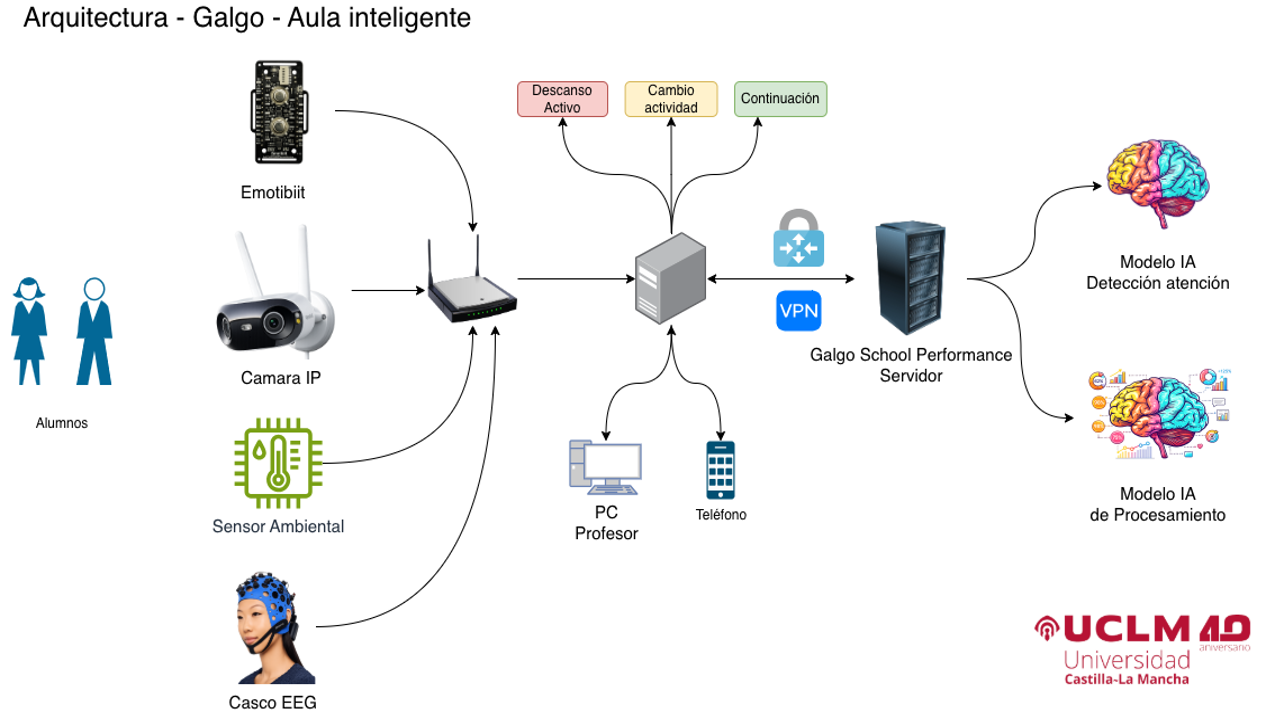
\includegraphics[width=\textwidth]{figuras/arquitectura_galgo.png}
    \caption{\textcolor{blue}{High-level architecture of the synchronised multimodal IoT platform. All sensing nodes are disciplined by a local Stratum-1 NTP server for sub-100~ms inter-modality alignment. Environmental, wearable and vision subsystems publish timestamped data to the MQTT broker; the on-server pipeline persists aggregated features for downstream analysis.}}
    \label{fig:architecture}
\end{figure}

\subsubsection{Environmental Mote: Custom PCB and Passive Ventilation}

Unlike generic commercial solutions, the environmental sensing node is built on a custom-designed multi-layer Printed Circuit Board (PCB) housing an ESP32 System-on-Chip (SoC). To guarantee measurement fidelity, the electronics are enclosed in a 3D-printed structure featuring a passive-ventilation duct system. This mechanical design effectively prevents the heat-island effect generated by the processor, a common source of systematic measurement bias in compact IoT devices. \textcolor{blue}{This node continuously samples temperature, relative humidity, equivalent CO$_2$, PM2.5, PM10, volatile organic compounds, illuminance, and sound pressure level.} The node samples at a nominal 15 Hz and aggregates per-second statistics. Audio is captured exclusively as dB SPL aggregates; no waveform is retained at any stage of the pipeline. The platform was developed within the UCLM teaching-innovation project “Aulas inteligentes para la mejora de la atención del estudiantado mediante algoritmos de Inteligencia Artificial integrados con visión artificial y tecnologías embebidas.” The link of indoor environmental quality to cognitive performance in school-age populations is established \parencite{Wargocki2007_effects,Bako2012_classroom,Satish2012_co2,Petersen2016_classroom,Mendell2013_ventilation,Allen2016_cogfx,Twardella2012_co2_classroom}; this modality contributes a per-window contextual variable, not a per-student feature.

\subsubsection{Wearable Biosignal Suite}

Physiological and neurophysiological data are captured through a non-invasive wearable suite \parencite{hong_advances_2025,HernandezMustieles2024_wearable_education}. First, six EmotiBit physiological wristbands record heart rate and heart-rate variability via photoplethysmography (PPG) at 25~Hz, electrodermal activity (EDA) at 15~Hz, peripheral skin temperature at 25~Hz, and 9-axis Inertial Measurement Unit (IMU) kinematics at 100~Hz continuously throughout each instrumented session \parencite{di_lascio_unobtrusive_2018, astudillo_capturing_2023}. Each unit is worn on the non-dominant forearm, an anatomical location that combines acceptable optical access for triple-wavelength photoplethysmography (PPG) with reduced exposure to writing-related motion artefacts in the dominant arm. Units rotate weekly across the consenting participants with sex-balanced random allocation so that a substantial fraction of the instrumented group has been recorded under standardised wear conditions over the four-month deployment. Each unit writes the session’s data to its on-board microSD card together with an \texttt{info.json} manifest. The choice of EmotiBit as the physiological layer is consistent with the team’s prior work on multimodal classification of cognitive states from physiological signals \parencite{SanchezReolid2024_eeg_fnirs}. 

Second, cortical activity is acquired via a 32-channel semi-dry Bitbrain Versatile Electroencephalography (EEG) system, recording at 256 Hz with 24-bit resolution. One participant per week is instrumented, selected by stratified random sampling that crosses academic-performance category with sex. The EEG session rotates across the four weekly Mathematics sessions and is aligned with the monthly Psychomotor Vigilance Task (PVT) administration when possible. This gel-free configuration allows for rapid placement by trained research personnel in the classroom, processing the power spectral density of the alpha, beta, and theta frequency bands \parencite{ramirez-moreno_eeg-based_2021, apicella_eeg-based_2022}. Semi-dry EEG matches conventional wet-gel EEG on many spectral and event-related features and is validated for adolescent populations \parencite{LopezGordo2014_dry_eeg,DiFlumeri2019_dry_eeg_validation,Hinrichs2020_motion_artifacts,LauZhu2019_mobile_eeg_review}. Procedures to mitigate the social-visibility of single-student instrumentation are described in \Cref{subsec:eeg-spotlight}.

\subsubsection{Classroom video for body-pose feature extraction}

A Reolink Elite Wi-Fi 4K dual-lens camera (180\textdegree\ horizontal field of view) is mounted near the ceiling above the blackboard. \textbf{Audio capture is disabled at the device-level configuration} (the configuration directive is documented in the Multimedia Appendix; \Cref{sec:appendix-privacy}). Video is processed exclusively on the institutional UCLM server to extract body-pose features (head, trunk and limb keypoints; head orientation; gross-motor activity; posture indicators) using established pose-estimation pipelines \parencite{Cao2021_openpose,Lugaresi2019_mediapipe,Sun2019_hrnet,Jocher2023_yolov8}. \textbf{The raw video file is deleted within 72 hours of feature extraction}, with a verifiable governance log capturing date, time, session identifier, responsible operator and deletion confirmation hash. Only the derived numeric features are retained.

\subsection{Outcomes and external validation instruments}\label{subsec:outcomes}

\subsubsection{Primary outcome: BOSS behavioural observation label}

\textcolor{blue}{The primary measure of cognitive performance is a 5-category behavioural annotation derived from the Behavioral Observation of Students in Schools (BOSS) system \parencite{Shapiro2011_boss,Volpe2023_classroom_observation_review,Alperin2023_boss_validation}. The annotation workflow operates in two stages. First, a transformer-like encoder on pose sequences processes the overhead video stream to detect segments where classroom dynamics change---defined as shifts in the spatial distribution or intensity of body-pose features (head orientation, gross-motor activity, posture changes) aggregated at the classroom level. The model outputs candidate event boundaries with associated timestamps. The model is validated on a held-out subset of the first two weeks of recordings against manually annotated transition points; the deployment threshold is set such that the false positive rate for event-boundary detection remains below 20\%.}

\textcolor{blue}{Second, an ad-hoc annotation application alerts the teacher when the model detects a dynamic change. The teacher assigns the flagged event one of five BOSS codes via the application interface: Active Engaged Time (AET: writing, hand-raising, interacting with materials), Passive Engaged Time (PET: sustained visual orientation toward the teacher, board, or screen), Off-Task Passive (OFT-P: staring into space, head on desk, disengagement without motor activity), Off-Task Motor (OFT-M: fidgeting, mobile phone use, unrelated manual activity), and Off-Task Verbal (OFT-V: talking or whispering about non-academic content). Each annotation records the event's start and end timestamps, producing state-event labels with associated durations. Because annotation is event-driven rather than fixed-interval, the teacher's burden is substantially lower than a continuous 5-minute schedule. The BOSS system has been validated in school-age populations \parencite{Alperin2023_boss_validation}, although most validation studies have been conducted in elementary education settings; its application to secondary education (ages 14--16) extends this evidence base and will contribute data on BOSS reliability in adolescent classroom contexts.}

\textcolor{blue}{Inter-rater reliability is assessed by having a second independent coder review a spot-check subset of video-recorded events and assign BOSS codes post hoc. Cohen's $\kappa$ between the teacher's in-session annotation and the second coder's post-hoc coding is reported as the primary label-reliability metric, testing H4.}

\subsubsection{Secondary outcome: end-of-session global rating}

The teacher records a 0--10 global rating of the class's attention/concentration at the end of every instrumented session. The secondary outcome serves to characterise within-teacher consistency between event-level annotation and lesson-level integration, and to validate the attention model's event-detection sensitivity against the teacher's holistic judgement.

\subsubsection{External-validation instrument: Psychomotor Vigilance Task}

The Psychomotor Vigilance Task (PVT) is administered via the \emph{Vigilance Buddy} iPad application in its validated 5-minute format, before and after a planned Mathematics session for both the instrumented and comparison groups, with monthly periodicity. Primary metrics are median and mean response time, number of lapses and slowest-10\% reaction time \parencite{Dinges1985_pvt,Loh2004_pvt_short,Basner2011_pvt,Basner2018_pvt_practice}. The PVT has been validated in school-age populations and is sensitive to within-day fluctuations in sustained attention in children and adolescents \parencite{Barel2022_pvt_children,Barel2022_sleep_pvt,GonzalezFernandez2023_pvt_breaks}. \textcolor{blue}{The PVT provides a participant-session-level external anchor for the BOSS-derived attentional labels; the convergent-validity relationship between objective vigilance and observed classroom behaviour is discussed in \Cref{subsec:construct-validity}.}

\subsubsection{Auxiliary measures and covariates}

Auxiliary measures are recorded at the cohort level: a sociodemographic questionnaire and the Spanish-validated PAQ-A self-report of physical activity \parencite{MartinezGomez2009_paq_a} are administered at the start and end of the study; objective physical activity is measured via ActiGraph wGT3X-BT for two weeks (one at the start, one at the end) with established cut-points \parencite{Evenson2008_actigraph}; and physical fitness is measured once during a Physical Education session through the ALPHA-Fitness battery \parencite{RuizFernandez2011_alpha}. The session-level covariates (subject, teacher identifier, date/time, instructional content, methodology, instructional style) are extracted from the teacher's session log.

\subsection{Data collection, time synchronisation and edge pipeline}\label{subsec:pipeline}

A critical challenge in in-the-wild multimodal deployments is the temporal alignment of heterogeneous data streams without tethering students to a central workstation \parencite{martinez-maldonado_lessons_2024}. To resolve this, all sensing nodes and the institutional UCLM server share a common time reference disciplined by the Network Time Protocol (NTP). All edge devices synchronize their internal Real-Time Clocks against a local Stratum-1 NTP server, generating timestamps at the exact microsecond of signal acquisition to decouple measurements from network jitter. The protocol target is sub-100 ms inter-modality alignment on the slow ambient channel and sub-50 ms alignment on EEG and video. \textcolor{blue}{Bench-test validation of this source-based timestamping mechanism under controlled conditions produced an end-to-end synchronisation error below 15 ms; in-deployment validation against the protocol target is described in the Method Validation plan (\Cref{subsec:method-validation}).}

Telemetry payloads from the sensors are published over the MQTT protocol to a local EMQX broker. \textcolor{blue}{To guarantee data integrity for high-frequency physiological time-series, the transport layer is configured to enforce MQTT Quality of Service level 2 (QoS 2), achieving exactly-once delivery during 60-minute continuous recording sessions.} The on-server pipeline then persists these per-window aggregated features to an InfluxDB time-series database for downstream supervised learning \parencite{Mishra2020_mqtt, Shi2016_edge}.

To mitigate cybersecurity risks during the transmission of sensitive biometric and behavioural data from the classroom to the institutional server, the edge pipeline incorporates a self-hosted Tailscale mesh network built upon the WireGuard protocol. This peer-to-peer mesh topology provides end-to-end encryption for the live data stream and simplifies the traversal of institutional firewalls without exposing any public endpoints, effectively mitigating the risk of packet interception or Man-in-the-Middle (MITM) attacks \parencite{alrashdi_ad-iot_2019}. \textcolor{blue}{Remote access to the institutional server by researchers is protected by a separate mutual-TLS VPN with multi-factor authentication, as documented in \Cref{sec:appendix-privacy}.}

Pseudonymisation is applied at the source: each participant is assigned an opaque identifier and the correspondence table between identifiers and personal data is kept encrypted and stored separately, accessible only to the principal investigator. No raw biometric or video data ever leave the institutional server; the operational details of the privacy-by-design pipeline and the automated deletion protocols are documented in \Cref{sec:appendix-privacy}.

\textcolor{blue}{\subsection{Data Analysis Plan}\label{subsec:analysis-plan}}

\textcolor{blue}{The analysis proceeds in four stages: per-modality signal processing and feature extraction, method validation, descriptive characterisation of the multimodal corpus, and predictive modelling via multimodal fusion. Stages 1--3 characterise the measurement infrastructure; stage 4 tests H2 and H3 using the model architectures pre-specified below.}

\textcolor{blue}{\subsubsection{Signal processing and feature extraction}}

\textcolor{blue}{Each modality is processed into per-event and per-window aggregated features. \textbf{Attention-based video event detection.} The overhead video stream is additionally processed by an attention-based temporal model that detects segments where classroom dynamics change. The model ingests per-frame body-pose feature sequences (head orientations, posture vectors, activity counts) and outputs candidate event boundaries where the spatial distribution or intensity of these features shifts beyond a learned threshold. These boundaries segment the continuous recording into behavioural events for subsequent BOSS annotation. The same body-pose features that serve the event detector are also aggregated per event as behavioural descriptors (mean head orientation, posture change rate, activity intensity) for downstream fusion.}

\textcolor{blue}{\textbf{Per-modality feature extraction.} Environmental telemetry (temperature, relative humidity, CO\textsubscript{2}, PM2.5, PM10, volatile organic compounds, illuminance, sound pressure level) is aggregated to per-window and per-event means, minima, maxima, and variances at the classroom level. EmotiBit signals are processed per participant: photoplethysmography yields heart rate and heart-rate variability indices (SDNN, RMSSD) via peak detection on the 25~Hz waveform; electrodermal activity is decomposed into tonic (skin conductance level) and phasic (skin conductance response count and amplitude) components; skin temperature is reduced to per-window mean and trend; 9-axis IMU data yield motion indices (activity counts, dominant frequency, and postural stability). EEG signals are bandpass-filtered (0.5--45~Hz), subjected to independent component analysis for artefact removal, and reduced to relative band power (delta 0.5--4~Hz, theta 4--8~Hz, alpha 8--13~Hz, beta 13--30~Hz, gamma 30--45~Hz) and inter-channel coherence per 5-minute window. Body-pose features are extracted from the overhead video stream using a fixed pose-estimation pipeline (e.g., YOLOv8-Pose \parencite{Jocher2023_yolov8}, MediaPipe \parencite{Lugaresi2019_mediapipe}, or HRNet \parencite{Sun2019_hrnet}), yielding per-window aggregates of head orientation, posture changes, gross-motor activity, and hand-raising event counts. All features are timestamped at acquisition and aligned to the 5-minute teacher-annotation windows.}

\textcolor{blue}{\subsubsection{Method validation}}

\textcolor{blue}{Before any inferential use, the measurement properties of each modality are validated against the criteria specified in \Cref{subsec:method-validation}: synchronisation latency and jitter via LED-flash testing; PPG--ECG agreement on a laboratory validation block; EEG impedance distribution and ICA-based artefact characterisation; body-pose detection mAP at IoU 0.5 and keypoint completeness; and environmental sensor drift against reference-instrument checks. The deployment is considered fit for subsequent analyses when the validation criteria are met.}

\textcolor{blue}{\subsubsection{Descriptive characterisation}}

\textcolor{blue}{The validated corpus is characterised through: (a)~per-modality data yield per session; (b)~per-modality missingness rate per event, stratified by modality and session; (c)~marginal and joint distributions of the BOSS label categories and the PVT change scores; and (d)~a session-level and participant-level correlation matrix (Spearman's $\rho$) between the four modality feature sets, the AET+PET engaged-time proportion, and the PVT change scores. BOSS inter-rater reliability is assessed via Cohen's $\kappa$ between the primary educational professional and a second independent coder on a spot-check subset of events. The comparison group is characterised in parallel. Group-level differences are reported as exploratory descriptors, not inferential contrasts.}

\textcolor{blue}{Missing data are handled in two stages. The per-modality missingness rate is reported as a primary quality metric. Descriptive tables and correlation matrices are computed on complete-case windows---those in which at least the teacher label and one physiological or behavioural modality are present. Windows missing the teacher label are excluded from correlation analyses. The proportion of excluded windows is reported alongside every statistic. Multiple imputation is deferred to the predictive modelling stage in subsequent compendium articles.}

\textcolor{blue}{\subsubsection{Multimodal fusion and predictive modelling}}

\textcolor{blue}{The per-window and per-event feature matrix is designed to train downstream multimodal machine learning models. Feature-level fusion concatenates modality-specific vectors into a single representation per event, which is fed to an XGBoost classifier as the primary model. Modality-specific models are trained in parallel for ablation and comparison: a 1D convolutional network on EEG time-frequency representations, and a temporal convolutional network on body-pose sequences. The predictions of these modality-specific models are aggregated via a logistic regression meta-learner trained on the BOSS label (5-class: AET, PET, OFT-P, OFT-M, OFT-V). The primary evaluation follows H2: the fused XGBoost model is tested against a label-shuffled baseline. Fusion gain (H3) is assessed by comparing the meta-learner against the best unimodal model. All models are evaluated under leave-one-student-out cross-validation with macro-averaged area under the precision-recall curve as the primary metric. For engaged-vs-off-task binary analyses, AET and PET are collapsed into a single engaged category and compared against the three off-task categories. Alternative architectures (e.g., LightGBM, transformer-based models) may be explored and are reported as secondary analyses. Full pre-analysis plans with exact hyperparameter configurations are declared in the subsequent compendium articles.}

\textcolor{blue}{\subsubsection{Sample size and expected data volume}}

\textcolor{blue}{The unit of analysis is the 5-minute window. The instrumented group attends four Mathematics sessions per week; the comparison group attends one. Over a four-month deployment ($\sim$16 teaching weeks) with approximately 50 minutes of recording per session ($\sim$10 windows), the expected data volume is:}

\textcolor{blue}{\begin{itemize}[leftmargin=*, itemsep=1pt]
  \item \textbf{Instrumented group:} $\sim$64 sessions, $\sim$640 labelled windows per participant, $\sim$16,000 total windows (assuming $\sim$25 students per class). Each window carries the full multimodal feature set: environmental aggregates, EmotiBit physiological features, body-pose features, and the binary teacher label.
  \item \textbf{Comparison group:} $\sim$16 sessions, $\sim$160 windows per participant, $\sim$4,000 total windows. These windows carry the teacher label, PVT scores, and session-level covariates only; no sensor data are collected.
  \item \textbf{EEG:} one participant per week ($\sim$16 individual EEG sessions across four months). Each session yields $\sim$10 windows of 32-channel EEG features, for approximately 160 EEG-labelled windows. The EEG sample size bounds neurophysiological inferences to the group level; participant-level EEG analyses are not attempted.
\end{itemize}}

\textcolor{blue}{This window-level granularity provides on the order of $10^3$--$10^4$ labelled instances for descriptive characterisation and, subsequently, for training and cross-validating the multimodal fusion models. The instrumented group's class-complete enrolment means the exact participant count is determined by consent uptake and reported in the data-release manifest. Statistical power for the participant-level PVT--teacher-label correlation and for the EEG group-level descriptives is reviewed in \Cref{subsec:limitations}.}

\subsection{Ethics and data governance}\label{subsec:ethics}

The study was designed and is conducted in accordance with the Declaration of Helsinki, the General Data Protection Regulation (Regulation (EU) 2016/679, GDPR) and the Spanish Organic Law 3/2018 on the Protection of Personal Data and Guarantee of Digital Rights (LOPDGDD). The protocol was submitted for review by the Ethics in Social Research Committee of the Universidad de Castilla-La Mancha (CEIS-UCLM); reference pending.

Participants are minors enrolled in 3rd and 4th of ESO, aged 14--16. Eligibility, consent and assent procedures are detailed in \Cref{subsec:recruitment}. The data collected (EEG, electrodermal activity, heart rate and heart-rate variability, body-pose features, behavioural observations) qualify as biometric and health-related data of minors and are therefore subject to the highest protection regime under GDPR Article 9 and LOPDGDD Article 9. Processing operations identified in this protocol are lawful under the explicit consent provision of GDPR Article 9(2)(a) and follow the data-protection-by-design and data-protection-by-default principles required by Article 25 \parencite{Macenaite2017_minors_gdpr,EDPB2020_consent}. The operational privacy pipeline (audio-disable configuration on the camera, 72-hour video-deletion governance log with confirmation hashes, pseudonymisation key management and access logging on the institutional server) is documented in \Cref{sec:appendix-privacy}.

\subsubsection{Visibility of participation in a class-complete deployment}\label{subsec:eeg-spotlight}

In a class-complete deployment, participating students wear a visible EmotiBit wristband during instrumented sessions, and one stratified-sampled student per week is also fitted with the Bitbrain Versatile EEG headset. The visibility of these devices may, in principle, function as a participation marker in front of peers and act as a behavioural spotlight on the EEG-instrumented student. The protocol mitigates this risk by (i) familiarising the whole class with the equipment during a single non-recorded introduction session at the start of the deployment, so that the devices stop being novel before recordings begin; (ii) rotating the EEG instrumentation across the four weekly Mathematics sessions and across academic-performance strata, so that the headset is not associated with any single subgroup; (iii) keeping the academic-performance stratification of the EEG sample confidential between the research team and the teacher leading the session, with no disclosure to peers or to the school's administration; and (iv) explicitly informing the EEG-instrumented student that the assignment is by random sampling within a balanced design and not by any individual academic feature. Residual social-comparison risk is acknowledged in \Cref{subsec:limitations}.

\subsubsection{Risks, benefits and special-category data of minors}

EmotiBit wristbands are worn on the non-dominant forearm and present negligible physical risk; participants may remove the device at any moment. The Bitbrain Versatile semi-dry EEG headset is fitted and removed by trained research personnel; immediate withdrawal is honoured if the participant reports discomfort. There is no direct benefit to the participants; the study informs future research on classroom-based cognitive-performance monitoring and the design of inclusive adaptive learning environments. Released artefacts (anonymised per-window aggregated features per modality, session-level metadata, analysis code) are deposited under restricted-access conditions consistent with the CEIS-UCLM approval; raw EEG, EmotiBit and ambient time series remain on the UCLM institutional server.

\subsection{Patient and public involvement}\label{subsec:ppi}

Students, parents and teaching staff are not formally involved in the design of this protocol because the design pre-dates the consent campaign and because the protocol implements an established multimodal sensing methodology rather than a novel intervention. The teacher who delivers the instrumented Mathematics sessions has participated in iterative refinement of the operational rule of the binary cognitive-performance label and of the Google Forms timing schedule, to ensure that the annotation task is compatible with ordinary classroom delivery. Participating students and their families receive a plain-language summary of the protocol, the data-governance arrangements and the withdrawal procedure at the moment of the consent-and-assent campaign. Aggregate-only findings will be returned to the participating school at the end of the doctoral compendium; no individual-level findings are returned to families, students, the school or the teaching staff.
